\documentclass[12pt]{article}
\usepackage[utf8]{inputenc}
\usepackage{geometry}
\geometry{a4paper, margin=1in}
\usepackage{tabularx}
\usepackage{enumitem}
\usepackage{booktabs}
\usepackage{xcolor}
\usepackage{titlesec}
\usepackage{hyperref}
\usepackage{caption}
\usepackage{float}
\usepackage{graphicx}
\usepackage{tikz}
\usepackage{longtable}
\usepackage{array}
\usepackage{amsmath}
\usepackage{listings}
\usepackage{fancyhdr}
\usepackage{setspace}
\usetikzlibrary{arrows.meta,positioning,shapes.geometric,calc}

\definecolor{mNavy}{RGB}{30,58,138}
\definecolor{mDark}{RGB}{15,23,42}
\definecolor{mSlate}{RGB}{71,85,105}
\definecolor{mBlue}{RGB}{37,99,235}
\definecolor{mPurple}{RGB}{124,58,237}
\definecolor{mGreen}{RGB}{5,150,105}
\definecolor{mOrange}{RGB}{234,88,12}
\definecolor{mLight}{RGB}{248,250,252}
\hypersetup{colorlinks=true,linkcolor=mDark,urlcolor=mBlue}
\captionsetup{labelfont={bf,color=mDark},font=small,skip=8pt}
\titleformat{\section}{\normalfont\Large\bfseries\color{mDark}}{\thesection}{1em}{}[\titlerule]
\titleformat{\subsection}{\normalfont\large\bfseries\color{mDark}}{\thesubsection}{1em}{}
\onehalfspacing
\pagestyle{fancy}
\fancyhf{}
\lhead{Event Collision Detector}
\rhead{Software Engineering Project Report}
\cfoot{\thepage}

\begin{document}

\begin{titlepage}
\begin{center}
\vspace*{1cm}
{\Large\textbf{THAPAR INSTITUTE OF ENGINEERING AND TECHNOLOGY}}\\[0.4em]
{\large Department of Computer Science and Engineering}\\[2cm]
{\Huge\textbf{Event Collision Detector}}\\[0.7em]
{\LARGE Predictive Launch-Window Intelligence}\\[2cm]
{\Large Software Engineering Project Report}\\[0.5em]
{\large Course Code: UCS503P}\\[2cm]
\begin{tabular}{ll}
\textbf{Submitted by:} & Jaskaran Singh\\
& Vaani Mehta\\
& Parmeet Singh\\[0.5em]
\textbf{Roll Numbers:} & 1024160033\\
& 1024160123\\
& 1024160021\\[0.5em]
\textbf{Submitted to:} & Jeelani Asif
\end{tabular}
\vfill
{\large Thapar Institute of Engineering and Technology, Patiala}\\
{\large September 2026}
\end{center}
\end{titlepage}

\pagenumbering{roman}
\section*{Declaration}
We hereby declare that this project report, titled ``Event Collision Detector: Predictive Launch-Window Intelligence,'' has been prepared as part of the Software Engineering course UCS503P. The report describes the proposed system, its requirements, architecture, design, implementation plan, and evaluation methodology. All project-specific assumptions and planned features are identified as such.

\section*{Acknowledgement}
We express our sincere gratitude to our course instructor, Jeelani Asif, for guidance and feedback throughout the development of this project proposal and report. We also acknowledge the support of Thapar Institute of Engineering and Technology and the Department of Computer Science and Engineering for providing the academic environment and resources required to undertake this work.

\section*{Abstract}
Selecting an appropriate launch date is an important decision for product and marketing teams because audience attention, media coverage, and promotional visibility are limited resources. Existing scheduling practices frequently focus on internal calendars and may overlook external events such as competitor announcements, industry conferences, entertainment programs, and major public occasions. This report presents the design of an Event Collision Detector, a web-based decision-support platform that aggregates external event intelligence, evaluates a proposed launch window, and recommends lower-risk alternatives.

The system uses a modular layered architecture comprising a React and Tailwind CSS client, a FastAPI application layer, a Python-based collision analysis service, an event-ingestion pipeline, PostgreSQL persistence, and Elasticsearch for low-latency date-range retrieval. The initial version uses explainable heuristic scoring based on temporal proximity, industry relevance, audience overlap, event magnitude, and media friction. Results are presented through an interactive dashboard containing a High, Medium, or Low risk classification, contributing events, and alternative launch dates.

The report defines functional and non-functional requirements, data models, use cases, data-flow descriptions, testing strategy, performance metrics, risks, and a phased implementation plan. The proposed evaluation targets a median collision-score latency of 500 milliseconds or less, at least 80 percent agreement with manually labelled assessments, and a recommendation quality of at least 90 percent. The project emphasizes rapid time-to-value, explainability, maintainability, and scalability while keeping the initial scope appropriate for an educational software engineering project.

\textbf{Keywords:} event intelligence, launch scheduling, collision detection, decision support, explainable scoring, Elasticsearch, FastAPI, React.

\tableofcontents
\newpage
\pagenumbering{arabic}

\section{Introduction}

\subsection{Background and Context}
Product launches and marketing campaigns do not occur in isolation. A company may plan a launch months in advance, prepare advertising material, coordinate public relations activities, and allocate a substantial budget to promotional channels. However, the success of the launch can be affected by events outside the company's internal control. A competitor may announce a similar product, a major technology conference may attract the same audience, or a high-profile public event may dominate media attention.

Traditional planning tools are effective at managing internal tasks, milestones, and dependencies, but they provide limited support for understanding the external attention landscape. Teams may manually search websites, social media, conference calendars, and news sources before choosing a date. Such a process is time-consuming, difficult to repeat consistently, and vulnerable to missing important events.

The Event Collision Detector addresses this gap by treating launch scheduling as an event-intelligence problem. It collects selected external events, normalizes them into a common representation, indexes them for efficient retrieval, and evaluates a proposed date against nearby activity. Instead of simply displaying a list of events, the platform converts the information into an actionable risk score and a set of alternative dates.

\subsection{Motivation}
The motivation for this project is the need for a practical and explainable method of reducing avoidable competition for attention. A scheduling tool should not replace managerial judgement; rather, it should provide evidence that helps users make better-informed decisions.

The system is particularly useful when:
\begin{itemize}[leftmargin=0.7cm]
\item a launch targets a clearly defined industry audience;
\item the marketing campaign depends on press coverage or social visibility;
\item several possible dates are available;
\item the cost of changing a launch date is lower than the cost of losing attention; and
\item decision-makers need an auditable explanation for why a date is considered risky.
\end{itemize}

\subsection{Problem Statement}
Marketing and product teams often choose launch dates using internal schedules without sufficient visibility into the external event landscape. This produces blind-spot scheduling, diluted audience attention, inefficient marketing expenditure, and an absence of systematic alternative-date discovery.

The problem can therefore be stated as follows:

\begin{quote}
How can a software system aggregate relevant external events and convert their temporal and contextual relationships into an explainable collision-risk assessment and practical launch-date recommendations?
\end{quote}

\subsection{Project Objectives}
\begin{enumerate}[leftmargin=0.7cm]
\item Aggregate event information from selected external sources and normalize it into a searchable event index.
\item Accept a proposed launch date, industry, audience, and related metadata.
\item Retrieve competing or attention-relevant events within a $\pm 7$ day window.
\item Compute an explainable collision-risk score using defined heuristic factors.
\item Search surrounding dates and recommend lower-risk launch windows.
\item Provide an interactive dashboard for reviewing scores, conflicts, and explanations.
\item Persist user submissions and finalized dates and establish a foundation for future calendar synchronization.
\end{enumerate}

\subsection{Scope}
The initial scope includes selected industries, structured event APIs, event normalization, date-window retrieval, heuristic scoring, recommendation generation, and dashboard visualization. The first implementation is expected to prioritize Technology and Entertainment or another limited set of industries selected by the team.

The project does not initially attempt to model every possible social trend, guarantee business outcomes, or replace human marketing decisions. Large-scale web scraping, advanced predictive modelling, and complete enterprise calendar management are outside the first iteration.

\subsection{Expected Contributions}
The project contributes a deployable software engineering prototype with:
\begin{itemize}[leftmargin=0.7cm]
\item a reusable event ingestion and normalization pipeline;
\item a low-latency searchable event index;
\item an explainable scoring service;
\item a recommendation workflow rather than a simple conflict list;
\item a dashboard suitable for non-technical users; and
\item a modular foundation for future data sources and predictive models.
\end{itemize}

\section{Literature and Existing-System Perspective}

\subsection{Existing Scheduling Practices}
Organizations commonly use internal calendars, project-management tools, spreadsheets, and team communication systems to coordinate launches. These systems are valuable for operational planning but are generally not designed to identify external competition for audience attention. Manual research can supplement them, but it often depends on individual experience and inconsistent search habits.

\subsection{Event Aggregation Platforms}
Public event APIs and event-discovery platforms provide structured information such as event titles, dates, locations, categories, and descriptions. These sources can reduce the effort required to gather information, although their coverage and metadata quality may vary. The proposed system therefore includes a normalization layer and source-management configuration rather than assuming that all providers use the same schema.

\subsection{Decision-Support Systems}
Decision-support systems combine data retrieval and analytical rules to help users evaluate alternatives. The Event Collision Detector follows this principle: it presents evidence, calculates a transparent score, and allows the user to compare alternative dates. The system is intended to support rather than automate final decision-making.

\subsection{Gap Addressed by the Proposed System}
The distinctive focus of the project is the combination of cross-industry event intelligence, temporal collision analysis, explainable scoring, and alternative-date discovery in a single workflow. The initial implementation deliberately uses understandable heuristics so that the output can be validated and discussed within a software engineering setting.

\section{Requirements Analysis}

\subsection{Stakeholders}
The primary stakeholders are:
\begin{itemize}[leftmargin=0.7cm]
\item \textbf{Product managers:} evaluate suitable dates for product announcements.
\item \textbf{Marketing teams:} assess potential competition for campaign visibility.
\item \textbf{Event planners:} identify conflicts with conferences and industry activities.
\item \textbf{Administrators:} configure industries, event sources, and user access.
\item \textbf{Developers and maintainers:} monitor ingestion, scoring, and system performance.
\end{itemize}

\subsection{Functional Requirements}
\begin{longtable}{p{0.17\textwidth}p{0.72\textwidth}}
\toprule
\textbf{ID} & \textbf{Requirement}\\
\midrule
FR-01 & The system shall allow a registered user to submit a proposed launch date.\\
FR-02 & The system shall accept relevant launch metadata such as industry and audience tags.\\
FR-03 & The ingestion service shall retrieve events from configured external sources.\\
FR-04 & The system shall normalize external events into a common schema.\\
FR-05 & The event index shall support date-range and category-based retrieval.\\
FR-06 & The scoring service shall calculate a collision-risk score for a proposed date.\\
FR-07 & The system shall classify the score as High, Medium, or Low risk.\\
FR-08 & The dashboard shall display the events contributing to the score.\\
FR-09 & The system shall search nearby dates for lower-risk alternatives.\\
FR-10 & The system shall store user submissions and finalized dates.\\
FR-11 & Administrators shall be able to configure supported industries and sources.\\
FR-12 & The system should support calendar synchronization in a subsequent release.\\
\bottomrule
\end{longtable}

\subsection{Non-Functional Requirements}
\begin{itemize}[leftmargin=0.7cm]
\item \textbf{Performance:} Median score latency should not exceed 500 ms for indexed queries.
\item \textbf{Availability:} Core dashboard and scoring functions should remain available during normal project demonstrations.
\item \textbf{Scalability:} Ingestion and scoring should be separable so that event volume can grow independently.
\item \textbf{Maintainability:} Modules should have clear responsibilities and documented API contracts.
\item \textbf{Usability:} A user should be able to submit a date and understand the result without technical knowledge.
\item \textbf{Security:} Authentication, session handling, and external OAuth credentials should be protected.
\item \textbf{Explainability:} Each risk result should identify the principal events and factors contributing to it.
\end{itemize}

\subsection{Assumptions and Constraints}
\begin{itemize}[leftmargin=0.7cm]
\item Initial event coverage will be limited to selected industries and available APIs.
\item External APIs may have rate limits, incomplete metadata, or changing schemas.
\item The first release will use heuristic scoring instead of requiring a trained predictive model.
\item Deployment must remain feasible on standard cloud infrastructure or containerized local environments.
\item Calendar synchronization may be implemented after the core workflow is stable.
\end{itemize}

\section{System Design}

\subsection{High-Level Architecture}
The system follows a five-layer architecture:
\begin{enumerate}[leftmargin=0.7cm]
\item Client tier for user interaction and visualization.
\item Application tier for REST APIs and authentication.
\item Analysis tier for collision scoring and recommendations.
\item Ingestion tier for external data retrieval and normalization.
\item Data tier for persistent user records and searchable event data.
\end{enumerate}

\begin{figure}[H]
\centering
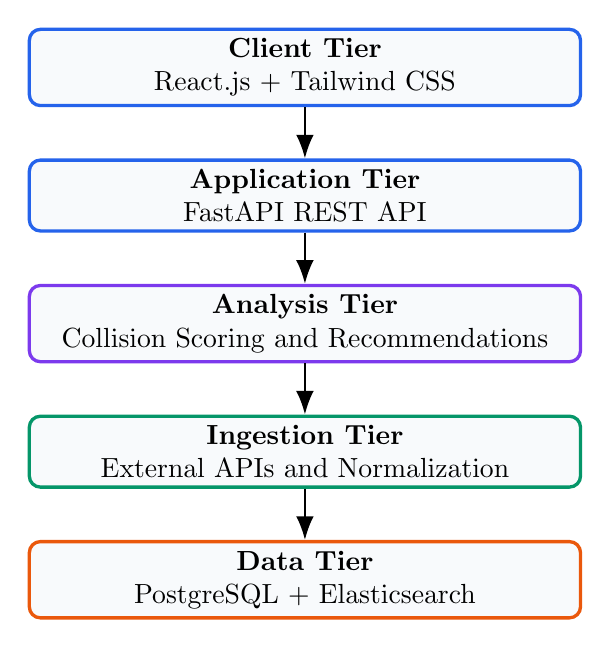
\begin{tikzpicture}[node distance=0.65cm]
\node[draw=mBlue,rounded corners,very thick,fill=mLight,minimum width=7cm,minimum height=0.9cm,align=center] (client) {\textbf{Client Tier}\\React.js + Tailwind CSS};
\node[draw=mBlue,rounded corners,very thick,fill=mLight,minimum width=7cm,minimum height=0.9cm,align=center,below=of client] (api) {\textbf{Application Tier}\\FastAPI REST API};
\node[draw=mPurple,rounded corners,very thick,fill=mLight,minimum width=7cm,minimum height=0.9cm,align=center,below=of api] (analysis) {\textbf{Analysis Tier}\\Collision Scoring and Recommendations};
\node[draw=mGreen,rounded corners,very thick,fill=mLight,minimum width=7cm,minimum height=0.9cm,align=center,below=of analysis] (ingest) {\textbf{Ingestion Tier}\\External APIs and Normalization};
\node[draw=mOrange,rounded corners,very thick,fill=mLight,minimum width=7cm,minimum height=0.9cm,align=center,below=of ingest] (data) {\textbf{Data Tier}\\PostgreSQL + Elasticsearch};
\draw[-{Latex[length=3mm]},thick] (client)--(api);
\draw[-{Latex[length=3mm]},thick] (api)--(analysis);
\draw[-{Latex[length=3mm]},thick] (analysis)--(ingest);
\draw[-{Latex[length=3mm]},thick] (ingest)--(data);
\end{tikzpicture}
\caption{Layered architecture of the Event Collision Detector}
\end{figure}

\subsection{Core Workflow}
The end-to-end workflow consists of six stages:
\begin{enumerate}[leftmargin=0.7cm]
\item \textbf{Ingest and normalize:} Scheduled jobs collect external events and transform them into a common format.
\item \textbf{Process submission:} A user submits launch details through the dashboard.
\item \textbf{Retrieve nearby events:} Elasticsearch returns events occurring within the defined time window.
\item \textbf{Compute risk and recommendations:} The analysis service applies scoring rules and compares alternative dates.
\item \textbf{Render dashboard:} The frontend displays the risk level, score breakdown, conflicts, and date cards.
\item \textbf{Sync confirmed date:} The selected date is stored and may later be pushed to Google or Outlook calendars.
\end{enumerate}

\subsection{Data Flow Description}
External event providers send raw records to the ingestion service. The service validates fields, converts dates to a consistent representation, maps categories to configured industries, removes duplicates where possible, and writes normalized records to Elasticsearch.

User launch submissions are sent to FastAPI and recorded in PostgreSQL. The API requests nearby events from Elasticsearch and passes the result to the scoring service. The scoring service returns a numerical score, classification, explanations, and ranked alternatives. The API sends this response to the React dashboard.

\subsection{Use Cases}
\begin{longtable}{p{0.18\textwidth}p{0.25\textwidth}p{0.43\textwidth}}
\toprule
\textbf{Use Case} & \textbf{Primary Actor} & \textbf{Description}\\
\midrule
UC-01 Submit Launch Date & Product Manager & Enter proposed date and launch metadata.\\
UC-02 View Risk Assessment & Product Manager & Review classification, score, and conflicting events.\\
UC-03 Compare Alternatives & Product Manager & Inspect nearby dates with lower risk.\\
UC-04 Manage Sources & Administrator & Configure industries and external event sources.\\
UC-05 Review User Records & Administrator & Manage users and finalized submissions.\\
UC-06 Sync Calendar & User & Push a confirmed date to an external calendar.\\
\bottomrule
\end{longtable}

\subsection{Database Design}
The PostgreSQL store contains the following conceptual entities:
\begin{itemize}[leftmargin=0.7cm]
\item \textbf{User:} user identifier, name, email, authentication information, and role.
\item \textbf{Session:} session identifier, user reference, creation time, and expiry.
\item \textbf{LaunchSubmission:} proposed date, industry, audience tags, status, and timestamps.
\item \textbf{FinalizedEvent:} selected date, user reference, calendar status, and synchronization metadata.
\end{itemize}

The Elasticsearch index contains:
\begin{itemize}[leftmargin=0.7cm]
\item external event identifier and source;
\item title and description;
\item start and end timestamps;
\item industry and category;
\item audience tags;
\item estimated event magnitude;
\item location and source URL where available; and
\item ingestion and update timestamps.
\end{itemize}

\section{Methodology and Implementation Plan}

\subsection{Development Methodology}
An iterative and incremental development methodology is proposed. Each iteration produces a demonstrable improvement to the system. The team will first establish the minimum viable workflow and then add features only after the core pipeline is stable.

\begin{enumerate}[leftmargin=0.7cm]
\item Requirements and scope definition.
\item Data-source investigation and schema design.
\item Backend API and database setup.
\item Event ingestion and indexing.
\item Scoring engine implementation.
\item Frontend dashboard development.
\item Integration, testing, and evaluation.
\item Documentation and deployment.
\end{enumerate}

\subsection{Event Ingestion Module}
The ingestion module retrieves records from configured event sources. Each source adapter is responsible for communicating with its provider and returning raw records. A normalization component converts these records into the internal event schema.

The normalization process includes:
\begin{enumerate}[leftmargin=0.7cm]
\item validating mandatory fields;
\item parsing and standardizing dates and time zones;
\item mapping source categories to internal industry labels;
\item extracting audience tags from structured fields or descriptions where available;
\item estimating event magnitude using configured source information; and
\item detecting duplicates using source identifiers and matching attributes.
\end{enumerate}

\subsection{Collision Scoring Module}
The scoring module evaluates each retrieved event relative to the proposed launch date. A conceptual weighted formulation is:

\[
S = w_tT + w_iI + w_aA + w_mM + w_fF
\]

where $T$ represents temporal proximity, $I$ represents industry relevance, $A$ represents audience overlap, $M$ represents event magnitude, and $F$ represents media friction. The weights $w_t,w_i,w_a,w_m,w_f$ can be configured and validated using labelled examples.

The score is then mapped to a risk category. The exact thresholds will be tuned during validation rather than treated as universal business constants. The dashboard will show both the category and the factors responsible for the result.

\subsection{Recommendation Module}
The recommendation module evaluates candidate dates around the proposed date. It retrieves relevant events for each candidate window, calculates the score, filters invalid or unavailable dates, and ranks the remaining candidates by risk. The output includes the recommended date, score, and a concise explanation.

\subsection{Frontend Module}
The frontend provides:
\begin{itemize}[leftmargin=0.7cm]
\item launch-date and metadata input forms;
\item risk summary cards;
\item event conflict lists;
\item factor-level explanations;
\item alternative-date comparison;
\item loading and error states; and
\item finalized-date and calendar actions.
\end{itemize}

\subsection{API Design}
Illustrative API endpoints are listed below.

\begin{longtable}{p{0.25\textwidth}p{0.2\textwidth}p{0.4\textwidth}}
\toprule
\textbf{Endpoint} & \textbf{Method} & \textbf{Purpose}\\
\midrule
/api/launches & POST & Submit a proposed launch date.\\
/api/launches/\{id\} & GET & Retrieve a saved submission and assessment.\\
/api/assessments/\{id\} & GET & Return score, conflicts, and explanations.\\
/api/recommendations & POST & Generate lower-risk alternative dates.\\
/api/events & GET & Query indexed events.\\
/api/admin/sources & GET/POST & Manage configured event sources.\\
/api/calendar/sync & POST & Synchronize a confirmed date in a later release.\\
\bottomrule
\end{longtable}

\subsection{Security and Privacy Considerations}
Authentication and authorization should restrict administrative functions and protect user records. Passwords must never be stored in plain text. OAuth tokens for calendar providers should be handled securely and should not be exposed to the frontend unnecessarily. External source data should be treated as untrusted input and validated before indexing.

The project should collect only information required for scheduling and account management. Logging should avoid exposing secrets, authentication tokens, or unnecessary personal information.

\section{Project Management}

\subsection{Team Responsibilities}
\begin{longtable}{p{0.25\textwidth}p{0.62\textwidth}}
\toprule
\textbf{Area} & \textbf{Suggested Responsibility}\\
\midrule
Frontend and UX & Dashboard, forms, visualization, and responsive interaction.\\
Backend and API & FastAPI services, authentication, validation, and integration.\\
Data and Scoring & Event schema, ingestion, Elasticsearch, and collision heuristics.\\
Testing and Documentation & Test plans, CI/CD, evaluation, diagrams, and report maintenance.\\
\bottomrule
\end{longtable}

Responsibilities may overlap, and all members should review the integrated system and documentation.

\subsection{Phased Timeline}
\begin{longtable}{p{0.18\textwidth}p{0.28\textwidth}p{0.42\textwidth}}
\toprule
\textbf{Phase} & \textbf{Activity} & \textbf{Deliverable}\\
\midrule
Phase 1 & Requirements and research & Scope, use cases, and schema\\
Phase 2 & Backend foundation & FastAPI, PostgreSQL, authentication\\
Phase 3 & Data pipeline & Source adapter, normalization, Elasticsearch\\
Phase 4 & Scoring engine & Risk calculation and explanations\\
Phase 5 & Frontend & Dashboard and submission workflow\\
Phase 6 & Integration & End-to-end working prototype\\
Phase 7 & Testing & Unit, integration, performance, usability tests\\
Phase 8 & Finalization & Deployment, documentation, and presentation\\
\bottomrule
\end{longtable}

\subsection{Risk Register}
\begin{longtable}{p{0.22\textwidth}p{0.25\textwidth}p{0.38\textwidth}}
\toprule
\textbf{Risk} & \textbf{Impact} & \textbf{Mitigation}\\
\midrule
API rate limits & Missing or delayed events & Cache records and schedule ingestion responsibly.\\
Incomplete source coverage & Underestimated collision risk & Display data limitations and support multiple sources.\\
Inconsistent metadata & Incorrect scoring & Normalize and validate records before indexing.\\
Heuristic inaccuracy & Poor recommendations & Tune weights against manually labelled examples.\\
Over-engineering & Delayed delivery & Limit first release to selected industries.\\
Integration failures & Broken workflow & Define API contracts and run continuous integration.\\
Credential exposure & Security incident & Use environment variables and secure token handling.\\
\bottomrule
\end{longtable}

\section{Results and Evaluation}

\subsection{Evaluation Strategy}
Because the project is being documented at the proposal and implementation-planning stage, this section defines planned measurements rather than claiming completed experimental results. The final report should replace planned values with measured values after implementation.

\subsection{Primary Metric: Collision Score Latency}
Collision Score Latency (CSL) is the elapsed time from a valid launch-date submission to the returned risk score and recommendation set.

The target is a median CSL of 500 milliseconds or less against the indexed Elasticsearch dataset. Backend request timing should be recorded for each request, and median, 95th percentile, minimum, and maximum values should be reported.

\subsection{Secondary Metrics}
\begin{itemize}[leftmargin=0.7cm]
\item \textbf{Scoring Agreement:} At least 80 percent agreement with manual assessments on a labelled validation set.
\item \textbf{Ingestion Freshness:} Newly published API events should appear in the event index within 24 hours of the scheduled ingestion cycle.
\item \textbf{Recommendation Quality:} At least 90 percent of returned recommendations should have a lower score than the original date.
\item \textbf{Dashboard Responsiveness:} Risk details should render within one second after the API response.
\item \textbf{Completeness:} Mandatory fields should be present in normalized event records.
\end{itemize}

\subsection{Test Cases}
\begin{longtable}{p{0.12\textwidth}p{0.48\textwidth}p{0.25\textwidth}}
\toprule
\textbf{ID} & \textbf{Test Case} & \textbf{Expected Result}\\
\midrule
TC-01 & Submit a valid future launch date. & Submission accepted and assessment generated.\\
TC-02 & Submit an invalid or missing date. & Validation error displayed.\\
TC-03 & Retrieve events within seven days before and after target. & Correct date window returned.\\
TC-04 & Evaluate a date with a major same-industry event. & Higher risk contribution recorded.\\
TC-05 & Evaluate a date with no relevant events. & Low-risk result or appropriately limited confidence.\\
TC-06 & Generate alternative dates. & Alternatives are ranked and explained.\\
TC-07 & Simulate unavailable external API. & Cached data or clear error handling used.\\
TC-08 & Verify unauthorized administrator request. & Access denied.\\
TC-09 & Submit duplicate event records. & Duplicate handling prevents unnecessary repetition.\\
TC-10 & Confirm frontend-backend contract. & Correct response rendered in dashboard.\\
\bottomrule
\end{longtable}

\subsection{Pilot Validation Plan}
Historical launch dates will be selected and manually researched for competing events. The manually prepared assessment will be compared with the system's classification and contributing factors. A small usability exercise will involve students role-playing marketing or product managers and completing representative tasks.

The validation process will record false positives, false negatives, unclear explanations, and cases where source coverage is insufficient. These observations will guide changes to weights, thresholds, metadata mapping, and user-interface wording.

\subsection{Expected Outcomes}
The expected result is a functional prototype that completes the date-input-to-recommendation workflow reliably. The system should demonstrate that event aggregation and indexed retrieval can support rapid, repeatable analysis while keeping the reasoning understandable.

The project is not expected to establish that a particular score guarantees commercial success. Instead, it aims to demonstrate measurable technical performance and useful decision support.

\section{Deployment and Maintenance}

\subsection{Deployment Architecture}
The application can be containerized into frontend, backend, ingestion, and supporting data services. PostgreSQL and Elasticsearch may be deployed using managed services or local containers during development. Environment variables should be used for API keys, database credentials, and OAuth configuration.

\subsection{Continuous Integration and Delivery}
GitHub Actions will be used to automate:
\begin{itemize}[leftmargin=0.7cm]
\item code linting;
\item unit and integration tests;
\item frontend build validation;
\item API contract checks;
\item documentation generation where applicable; and
\item deployment packaging.
\end{itemize}

\subsection{Monitoring and Maintenance}
The deployed system should log ingestion success, source failures, API latency, scoring errors, and index freshness. Monitoring should help identify stale event data and failing integrations before they affect user decisions. Maintenance activities include updating source adapters, reviewing scoring weights, managing index growth, and periodically validating recommendations.

\section{Discussion}

\subsection{Strengths}
The proposed architecture separates responsibilities clearly and allows the team to deliver a useful prototype without depending on advanced machine learning. Explainability is a major strength because users can inspect the events and factors behind a risk classification. The dual-store design also separates transactional records from search-oriented event retrieval.

\subsection{Limitations}
The quality of the system depends on the completeness and accuracy of external event sources. Heuristic scoring may not capture every factor influencing audience attention. Industry relevance and audience overlap can be difficult to infer from inconsistent metadata. Calendar synchronization and broad international event coverage introduce additional complexity.

These limitations are acceptable for the first iteration but should be communicated clearly in the dashboard and final evaluation.

\subsection{Future Enhancements}
Future versions may introduce:
\begin{enumerate}[leftmargin=0.7cm]
\item additional event providers and industries;
\item improved entity and audience classification;
\item historical learning from user-labelled outcomes;
\item machine-learning or statistical models after sufficient data is collected;
\item richer media and social-attention signals;
\item Google Calendar and Microsoft Outlook synchronization;
\item administrator analytics for source quality and system usage; and
\item scalable caching and distributed ingestion workers.
\end{enumerate}

\section{Conclusion}

\subsection{Summary of Work}
The Event Collision Detector is a proposed scheduling-intelligence platform designed to help teams avoid launching into crowded attention windows. It addresses a practical problem by combining external event aggregation, normalization, indexed retrieval, explainable collision scoring, and alternative-date recommendations.

The system uses React and Tailwind CSS for the dashboard, FastAPI for application services, Python for analysis, PostgreSQL for user and finalized-event records, and Elasticsearch for event search. Its modular architecture supports iterative development and future scalability.

\subsection{Key Findings}
The project proposal establishes that:
\begin{itemize}[leftmargin=0.7cm]
\item external event visibility can complement internal launch planning;
\item explainable heuristics are suitable for an initial educational prototype;
\item separating ingestion and scoring improves maintainability;
\item alternative-date recommendations provide greater practical value than conflict alerts alone; and
\item measurable latency, agreement, freshness, and recommendation metrics provide a concrete evaluation framework.
\end{itemize}

\subsection{Final Remarks}
The Event Collision Detector demonstrates the application of software engineering principles to a decision-support problem involving heterogeneous data, modular services, and user-facing analytics. The first release is intentionally constrained to deliver a reliable and understandable core workflow. With additional data sources, validation, and future predictive capabilities, the platform can evolve into a more comprehensive launch-planning assistant.

\section*{References}
\begin{enumerate}[leftmargin=0.7cm]
\item FastAPI Documentation. FastAPI framework for building APIs with Python.
\item React Documentation. React library for building user interfaces.
\item Elasticsearch Documentation. Elasticsearch search and analytics engine.
\item PostgreSQL Documentation. PostgreSQL relational database system.
\item GitHub Actions Documentation. Continuous integration and delivery workflows.
\end{enumerate}

\end{document}
